% Version 1

\documentclass[10pt]{llncs}

\usepackage{ucs}
\usepackage[utf8]{inputenc}
\usepackage{amsmath}
\usepackage{amsfonts}

\let\proof\relax
\let\endproof\relax

\usepackage{mathtools}
\usepackage{amsthm}
\usepackage{stmaryrd}
\usepackage{tikz}
\usetikzlibrary{calc}
\usepackage[noend]{algpseudocode}
\usepackage{algorithm}
\usepackage{xcolor}
\usepackage{graphicx}
\usepackage{multirow}
\usepackage{changepage}
\usepackage{todonotes}
\usepackage{comment}
\usepackage{blkarray}
\usepackage[symbol]{footmisc}
\usepackage[tableposition=top]{caption}
\usepackage[left=2.5cm,right=2.5cm]{geometry}

\usepackage{placeins}

\let\Oldsection\section
\renewcommand{\section}{\FloatBarrier\Oldsection}

\let\Oldsubsection\subsection
\renewcommand{\subsection}{\FloatBarrier\Oldsubsection}

\let\Oldsubsubsection\subsubsection
\renewcommand{\subsubsection}{\FloatBarrier\Oldsubsubsection}


\newcommand{\QQIF}[1] {\State \textbf{if} (#1)}
\newcommand{\QQRETURN} {\textbf{return} }

\title{The Maximum Matrix Contraction problem : Appendix}
\author{
	Dimitri Watel\inst{1,2}
\and
	Pierre-Louis Poirion\inst{1,3}}
\institute{
 CEDRIC-CNAM, 292 rue du faubourg Saint Martin, 75003, Paris, FRANCE
\and
 ENSIIE, 1 Square de la résistance, Evry, FRANCE
  \email{dimitri.watel@ensiie.fr, }
\and
ENSTA Paristech, 828 boulevard des Maréchaux, 91120, Palaieau, FRANCE
\email{pierre-louis.poirion@ensta-paristech.fr}
}

\usepackage{caption}
\captionsetup[table]{aboveskip=5pt, }

\setcounter{secnumdepth}{3}


\newcommand{\gridsize}{0.5}
\newcommand{\prgrid}[3]{\draw[step=\gridsize,gray,very thin] (#1) grid (\gridsize*#3,\gridsize*#2);}
\newcommand{\prtline}[3]{}%\draw[] ($(#1)+(0,\gridsize*#2)$) -- ($(#1)+(\gridsize*#3,\gridsize*#2)$);}
\newcommand{\prtcolumn}[3]{}%\draw[] ($(#1)+(\gridsize*#2,0)$) -- ($(#1)+(\gridsize*#2,\gridsize*#3)$);}
\newcommand{\prvtline}[3]{\draw[very thick] ($(#1)+(0,\gridsize*#2)$) -- ($(#1)+(\gridsize*#3,\gridsize*#2)$);}
\newcommand{\prvtcolumn}[3]{\draw[very thick] ($(#1)+(\gridsize*#2,0)$) -- ($(#1)+(\gridsize*#2,\gridsize*#3)$);}
\newcommand{\prvtdline}[3]{\draw[very thick,dotted] ($(#1)+(0,\gridsize*#2)$) -- ($(#1)+(\gridsize*#3,\gridsize*#2)$);}
\newcommand{\prvtdcolumn}[3]{\draw[very thick,dotted] ($(#1)+(\gridsize*#2,0)$) -- ($(#1)+(\gridsize*#2,\gridsize*#3)$);}

\newcommand{\prvtdlinec}[4]{\draw[very thick,dotted,color=#4] ($(#1)+(0,\gridsize*#2)$) -- ($(#1)+(\gridsize*#3,\gridsize*#2)$);}
\newcommand{\prvtdcolumnc}[4]{\draw[very thick,dotted,color=#4] ($(#1)+(\gridsize*#2,0)$) -- ($(#1)+(\gridsize*#2,\gridsize*#3)$);}

\newcommand{\prvtrectc}[6]{\draw[very thick,color=#6] ($(#1)+(#3*\gridsize,#2*\gridsize)$) rectangle ($(#1)+(#5*\gridsize,#4*\gridsize)$);}

\newcommand{\prone}[3]{\draw ($(#1)+(#3*\gridsize-0.5*\gridsize,#2*\gridsize-0.5*\gridsize)$) node {$1$};}
\newcommand{\pronec}[4]{\draw[color=#4] ($(#1)+(#3*\gridsize-0.5*\gridsize,#2*\gridsize-0.5*\gridsize)$) node {$1$};}


\renewenvironment{comment}{\begingroup\sffamily\color{red} \itshape}{\endgroup}
\newcommand{\transpose}[1]{\ensuremath{#1^{\scriptscriptstyle T}}}

\renewcommand{\thefootnote}{\fnsymbol{footnote}}

\begin{document}




\theoremstyle{plain}
\newtheorem{corol}{Corollary}

\maketitle

\begin{abstract}
This document is an appendix of \cite{WP16}. In this paper, we introduce the {\it Maximum Matrix Contraction problem}, where we aim to contract as much as possible a binary matrix in order to maximize its density.  We prove this problem to be NP-Complete and that every algorithm solving this problem is at most a $2\sqrt{n}$-approximation algorithm where $n$ is the number of ones in the matrix. In this appendix, for each of the three heuristic algorithms proposed in \cite{WP16}, we give an instance proving the approximation ratio of that algorithm is not better than $O(\sqrt{n})$.
\textit{Keywords:} Complexity, Approximation algorithm, Linear Programming
\end{abstract}

This document contains the appendix of a paper accepted at the conference ISCO 2016, this appendix could not be added to the camera-ready version due to lack of space.

\appendix

We first briefly recall the definition of the Maximum Matrix contraction problem (MMC) introduced in \cite{WP16}. We are given a binary matrix (in which some entries contain a one and others contains a zero). Two lines $i$ and $i+1$ of the grid can be contracted by shifting up every one of line $i+1$ and of every line after. Two columns $j$ and $j+1$ of the grid can be contracted by shifting left the corresponding ones. However, such a contraction is not allowed if two ones are brought into the same entry. The purpose is to maximize the number of neighbor pairs of ones (including the diagonal ones). The measure is called the \emph{density} of the matrix. An illustration is given in Figure~\ref{fig:introduction:example}. 

\begin{figure}[!ht]
	\center
  \scalebox{0.7}{
	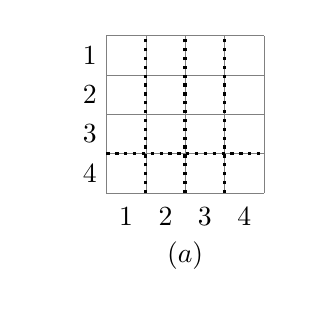
\begin{tikzpicture}
		\coordinate (O) at (0,0);
		
		\clip (-1,-1.25) rectangle (2.5,2.1);
		
		\prgrid{O}{4}{4}
		
		\prvtdline{O}{1}{4};
		
		\prvtdcolumn{O}{1}{4};
		\prvtdcolumn{O}{2}{4};
		\prvtdcolumn{O}{3}{4};
		
		\prbul{O}{1}{2}
		\prbul{O}{1}{4}
		\prbul{O}{2}{3}
		\prbul{O}{3}{1}
		\prbul{O}{3}{3}
		\prbul{O}{4}{1}
		
		
		\draw ($(O)+(-0,0.25)$) node[anchor=east] {$4$};
		\draw ($(O)+(-0,0.75)$) node[anchor=east] {$3$};
		\draw ($(O)+(-0,1.25)$) node[anchor=east] {$2$};
		\draw ($(O)+(-0,1.75)$) node[anchor=east] {$1$};
		
		\draw ($(O)+(0.25,-0.3)$) node {$1$};
		\draw ($(O)+(0.75,-0.3)$) node {$2$};
		\draw ($(O)+(1.25,-0.3)$) node {$3$};
		\draw ($(O)+(1.75,-0.3)$) node {$4$};
		
		\draw ($(O)+(1,-0.8)$) node {$(a)$};
		
	\end{tikzpicture}
	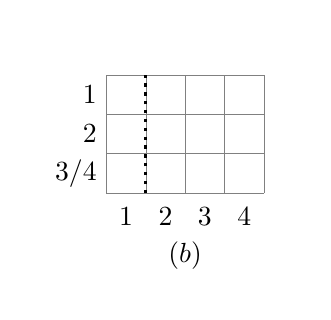
\begin{tikzpicture}
	\coordinate (O) at (0,0);
	
	\clip (-1,-1.25) rectangle (2.5,2.1);
	
	\prgrid{O}{3}{4}
	
	\prbul{O}{1}{2}
	\prbul{O}{1}{3}
	\prbul{O}{1}{4}
	\prbul{O}{2}{1}
	\prbul{O}{2}{3}
	\prbul{O}{3}{1}
		
	\prvtdcolumn{O}{1}{3};
	
	
	\draw ($(O)+(-0,0.25)$) node[anchor=east] {$3/4$};
	\draw ($(O)+(-0,0.75)$) node[anchor=east] {$2$};
	\draw ($(O)+(-0,1.25)$) node[anchor=east] {$1$};
	
	\draw ($(O)+(0.25,-0.3)$) node {$1$};
	\draw ($(O)+(0.75,-0.3)$) node {$2$};
	\draw ($(O)+(1.25,-0.3)$) node {$3$};
	\draw ($(O)+(1.75,-0.3)$) node {$4$};
	\draw ($(O)+(1,-0.8)$) node {$(b)$};
	\end{tikzpicture}
	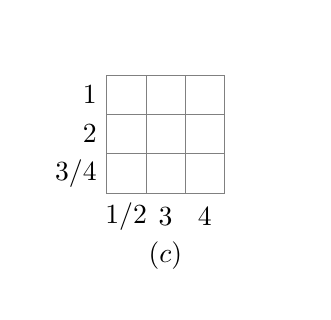
\begin{tikzpicture}
	\coordinate (O) at (0,0);
	
	\clip (-1,-1.25) rectangle (2.5,2.1);
	
	\prgrid{O}{3}{3}
	
	\prbul{O}{1}{1}
	\prbul{O}{1}{2}
	\prbul{O}{1}{3}
	\prbul{O}{2}{1}
	\prbul{O}{2}{2}
	\prbul{O}{3}{1}
	
	
	\draw ($(O)+(-0,0.25)$) node[anchor=east] {$3/4$};
	\draw ($(O)+(-0,0.75)$) node[anchor=east] {$2$};
	\draw ($(O)+(-0,1.25)$) node[anchor=east] {$1$};
	
	\draw ($(O)+(0.25,-0.3)$) node {$1/2$};
	\draw ($(O)+(0.75,-0.3)$) node {$3$};
	\draw ($(O)+(1.25,-0.3)$) node {$4$};
	\draw ($(O)+(0.75,-0.8)$) node {$(c)$};
	
	\end{tikzpicture}
  }
	\caption{In Figure~\ref{fig:introduction:example}.a, we give a $4 \times 4$ grid containing 6 dots. Valid contractions are represented by dotted lines and columns. It is not allowed to contract lines 1 and 2 because the two dots (1;1) and (2;1) would be brought into the same entry. Figure~\ref{fig:introduction:example}.b is the result of the contraction of lines 3 and 4 and Figure~\ref{fig:introduction:example}.c is the contraction of columns 1 and 2. The number of neighbor pairs in each grid is respectively 4, 7 and 10.
  }
	\label{fig:introduction:example}
\end{figure}
\vspace{-0.3cm}


In \cite{WP16}, we give three polynomial time heuristic algorithms for (MMC).
\begin{itemize}
	\item The greedy algorithm in which, at each iteration, we choose the line or column maximizing the increase of density of the matrix.
	\item The LCL algorithm which computes two maximally contracted matrices: the LC solution, in which we first contract a maximal set of lines and then contract a maximal set of columns; and the CL solution, in which we start with the columns and end with the lines. The LCL algorithm returns the solution with maximum density.
	\item The neighborization algorithm in which, at each iteration, we search for the line or the column such that the contraction of that line or column minimally decreases the number of pairs of 1 that can become neighbors. 
\end{itemize}
We prove in \cite{WP16} that those three algorithms are $2\sqrt{n}$-approximation algorithms.

The next section is dedicated to giving an example of instance in which there is a $O(\sqrt{n})$ ratio between the density of an optimal solution and the density of the worst feasible solution, where $n$ is the number of ones in the matrix. Each of the three subsections adapts that instance in order to prove that the approximation ratio of each of the three previous algorithms is not better than $O(\sqrt{n})$.

The last section gives a conjecture. 


\section{An instance with an $O(\sqrt{n})$ gap between the worst and the best solution.}

\label{apx:badinstance}


Theorem~\ref{theo:sqrtnapprox} of Section~\ref{sect:approx} proves a default $2\sqrt{n}$ upper bound of the approximation ratio for every algorithm returning a maximal solution.

We give, in this appendix, in Figure~\ref{fig:badinstance}, an instance in which the ratio between an optimal density and the lowest density of a maximal solution is at least $4\sqrt{n}$.

\begin{figure}
    \centering

    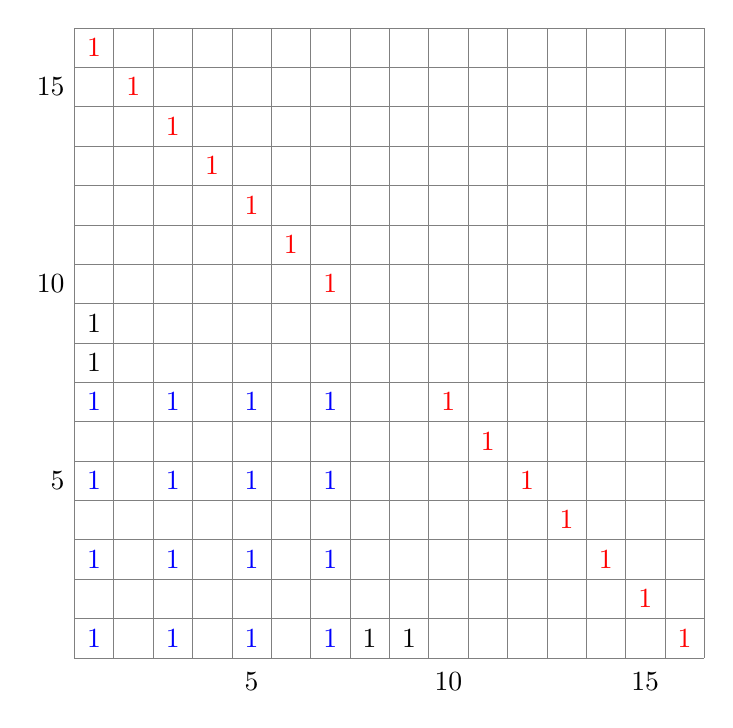
\begin{tikzpicture}
        \coordinate (O) at (0,0);
        \prgrid{O}{16}{16}

\definecolor{tempcolor}{rgb}{0.0,0.0,1.0}
        \pronec{O}{1}{1}{tempcolor};
\definecolor{tempcolor}{rgb}{0.0,0.0,1.0}
        \pronec{O}{1}{3}{tempcolor};
\definecolor{tempcolor}{rgb}{0.0,0.0,1.0}
        \pronec{O}{1}{5}{tempcolor};
\definecolor{tempcolor}{rgb}{0.0,0.0,1.0}
        \pronec{O}{1}{7}{tempcolor};
\definecolor{tempcolor}{rgb}{0.0,0.0,0.0}
        \pronec{O}{1}{8}{tempcolor};
\definecolor{tempcolor}{rgb}{0.0,0.0,0.0}
        \pronec{O}{1}{9}{tempcolor};
\definecolor{tempcolor}{rgb}{1.0,0.0,0.0}
        \pronec{O}{1}{16}{tempcolor};

\definecolor{tempcolor}{rgb}{1.0,0.0,0.0}
        \pronec{O}{2}{15}{tempcolor};

\definecolor{tempcolor}{rgb}{0.0,0.0,1.0}
        \pronec{O}{3}{1}{tempcolor};
\definecolor{tempcolor}{rgb}{0.0,0.0,1.0}
        \pronec{O}{3}{3}{tempcolor};
\definecolor{tempcolor}{rgb}{0.0,0.0,1.0}
        \pronec{O}{3}{5}{tempcolor};
\definecolor{tempcolor}{rgb}{0.0,0.0,1.0}
        \pronec{O}{3}{7}{tempcolor};
\definecolor{tempcolor}{rgb}{1.0,0.0,0.0}
        \pronec{O}{3}{14}{tempcolor};

\definecolor{tempcolor}{rgb}{1.0,0.0,0.0}
        \pronec{O}{4}{13}{tempcolor};

\definecolor{tempcolor}{rgb}{0.0,0.0,1.0}
        \pronec{O}{5}{1}{tempcolor};
\definecolor{tempcolor}{rgb}{0.0,0.0,1.0}
        \pronec{O}{5}{3}{tempcolor};
\definecolor{tempcolor}{rgb}{0.0,0.0,1.0}
        \pronec{O}{5}{5}{tempcolor};
\definecolor{tempcolor}{rgb}{0.0,0.0,1.0}
        \pronec{O}{5}{7}{tempcolor};
\definecolor{tempcolor}{rgb}{1.0,0.0,0.0}
        \pronec{O}{5}{12}{tempcolor};

\definecolor{tempcolor}{rgb}{1.0,0.0,0.0}
        \pronec{O}{6}{11}{tempcolor};

\definecolor{tempcolor}{rgb}{0.0,0.0,1.0}
        \pronec{O}{7}{1}{tempcolor};
\definecolor{tempcolor}{rgb}{0.0,0.0,1.0}
        \pronec{O}{7}{3}{tempcolor};
\definecolor{tempcolor}{rgb}{0.0,0.0,1.0}
        \pronec{O}{7}{5}{tempcolor};
\definecolor{tempcolor}{rgb}{0.0,0.0,1.0}
        \pronec{O}{7}{7}{tempcolor};
\definecolor{tempcolor}{rgb}{1.0,0.0,0.0}
        \pronec{O}{7}{10}{tempcolor};

\definecolor{tempcolor}{rgb}{0.0,0.0,0.0}
        \pronec{O}{8}{1}{tempcolor};

\definecolor{tempcolor}{rgb}{0.0,0.0,0.0}
        \pronec{O}{9}{1}{tempcolor};

\definecolor{tempcolor}{rgb}{1.0,0.0,0.0}
        \pronec{O}{10}{7}{tempcolor};

\definecolor{tempcolor}{rgb}{1.0,0.0,0.0}
        \pronec{O}{11}{6}{tempcolor};

\definecolor{tempcolor}{rgb}{1.0,0.0,0.0}
        \pronec{O}{12}{5}{tempcolor};

\definecolor{tempcolor}{rgb}{1.0,0.0,0.0}
        \pronec{O}{13}{4}{tempcolor};

\definecolor{tempcolor}{rgb}{1.0,0.0,0.0}
        \pronec{O}{14}{3}{tempcolor};

\definecolor{tempcolor}{rgb}{1.0,0.0,0.0}
        \pronec{O}{15}{2}{tempcolor};

\definecolor{tempcolor}{rgb}{1.0,0.0,0.0}
        \pronec{O}{16}{1}{tempcolor};

\draw ($(O)+(0,2.25)$) node[anchor=east] {$5$};
\draw ($(O)+(0,4.75)$) node[anchor=east] {$10$};
\draw ($(O)+(0,7.25)$) node[anchor=east] {$15$};
\draw ($(O)+(2.25,-0.3)$) node {$5$};
\draw ($(O)+(4.75,-0.3)$) node {$10$};
\draw ($(O)+(7.25,-0.3)$) node {$15$};

    \end{tikzpicture}
    \caption{An example of grid in which the gap between an optimal solution and the worst maximal solution is $O(\sqrt{n})$.}
    \label{fig:badExample}
\end{figure}


We highly believe this instance is the worst case that can happen and that the density of a maximal solution is always higher than $4\sqrt{n}$. The result of Theorem~\ref{theo:sqrtnapprox} may then possibly be updated to the following conjecture. 

\begin{conjecture}
	An algorithm returning any maximal solution of an instance of MMC is a $\sqrt{n}$-approximation.
\end{conjecture}

\bibliographystyle{acm}
\bibliography{edla}

\end{document}